\documentclass[12pt]{article}
\usepackage{url, graphicx, epstopdf, amsmath, esint}
\usepackage{physics}

% page layout
\setlength{\topmargin}{-0.25in}
\setlength{\textheight}{9.5in}
\setlength{\headheight}{0in}
\setlength{\headsep}{0in}
\setlength{\parindent}{1.1\baselineskip}
\addtolength{\oddsidemargin}{-0.75in}
\setlength{\marginparwidth}{2in}

% problem formatting
\newcommand{\problemname}{Problem}
\newcounter{problem}
\newcommand{\startproblem}{\paragraph{Problem~\theproblem:}\refstepcounter{problem}}

% words
\newcommand{\foreign}[1]{\textsl{#1}}
\newcommand{\vs}{\foreign{vs}}

% math
\renewcommand{\vec}[1]{\boldsymbol{#1}}
% \newcommand{\dd}{\mathrm{d}} % PROVIDED IN physics PACKAGE
\newcommand{\e}{\mathrm{e}}
% \newcommand{\cross}{\times} % PROVIDED IN physics PACKAGE
% \newcommand{\curl}{\vec{\nabla}\times} % PROVIDED IN physics PACKAGE

% primary units
\newcommand{\rad}{\mathrm{rad}}
\newcommand{\kg}{\mathrm{kg}}
\newcommand{\m}{\mathrm{m}}
\newcommand{\s}{\mathrm{s}}
\newcommand{\A}{\mathrm{A}}

% secondary units
\renewcommand{\deg}{\mathrm{deg}}
\newcommand{\km}{\mathrm{km}}
\newcommand{\cm}{\mathrm{cm}}
\newcommand{\mm}{\mathrm{mm}}
\newcommand{\mum}{\mathrm{\mu m}}
\newcommand{\nm}{\mathrm{nm}}
\newcommand{\ft}{\mathrm{ft}}
\newcommand{\mi}{\mathrm{mi}}
\newcommand{\AU}{\mathrm{AU}}
\newcommand{\ns}{\mathrm{ns}}
\newcommand{\h}{\mathrm{h}}
\newcommand{\yr}{\mathrm{yr}}
\newcommand{\N}{\mathrm{N}}
\newcommand{\J}{\mathrm{J}}
\newcommand{\eV}{\mathrm{eV}}
\newcommand{\MeV}{\mathrm{MeV}}
\newcommand{\W}{\mathrm{W}}
\newcommand{\Pa}{\mathrm{Pa}}
\newcommand{\C}{\mathrm{C}}
\newcommand{\V}{\mathrm{V}}
\newcommand{\ohm}{\mathrm{\Omega}}
\newcommand{\muF}{\mathrm{\mu F}}
\newcommand{\Hz}{\mathrm{Hz}}
\newcommand{\GHz}{\mathrm{GHz}}

% derived units
\newcommand{\mps}{\m\,\s^{-1}}
\newcommand{\mph}{\mi\,\h^{-1}}
\newcommand{\mpss}{\m\,\s^{-2}}
\newcommand{\radps}{\rad\,\s^{-1}}

% random stuff
\sloppy\sloppypar\raggedbottom\frenchspacing\thispagestyle{empty}

\begin{document}

\section*{NYU Physics 2---Problem Set 6}

Due Thursday 2020 March 12 at the beginning of lecture.

\paragraph{Problem~\theproblem:}\refstepcounter{problem}%
What is the density of conduction electrons in copper wire?  Give your
answer in $\mathrm{cm^{-3}}$.  Look up the density of copper and its
atomic weight, and imagine that there is one conduction electron per
atom (ie, all the other electrons are bound to the nuclei).  A good
car battery can put out about $250~\mathrm{A\,h}$ of total charge at
$12~\mathrm{V}$.  If you simply short-out your car battery with a
copper wire of diameter $5~\mathrm{mm}$, how far does a typical
conduction electron move in the wire? Don't do the experiment! It's
incredibly dangerous.

\paragraph{Problem~\theproblem:}\refstepcounter{problem}%
In this circuit, resistor $R_3$ is variable; that is, you can tune it. At what value of $R_3$
is the current through resistor $R$ exactly zero? What happens if $R_3$ is
greater than this resistance? Which way does the current flow through resistor $R$ and what is
the magnitude of the current?
\marginpar{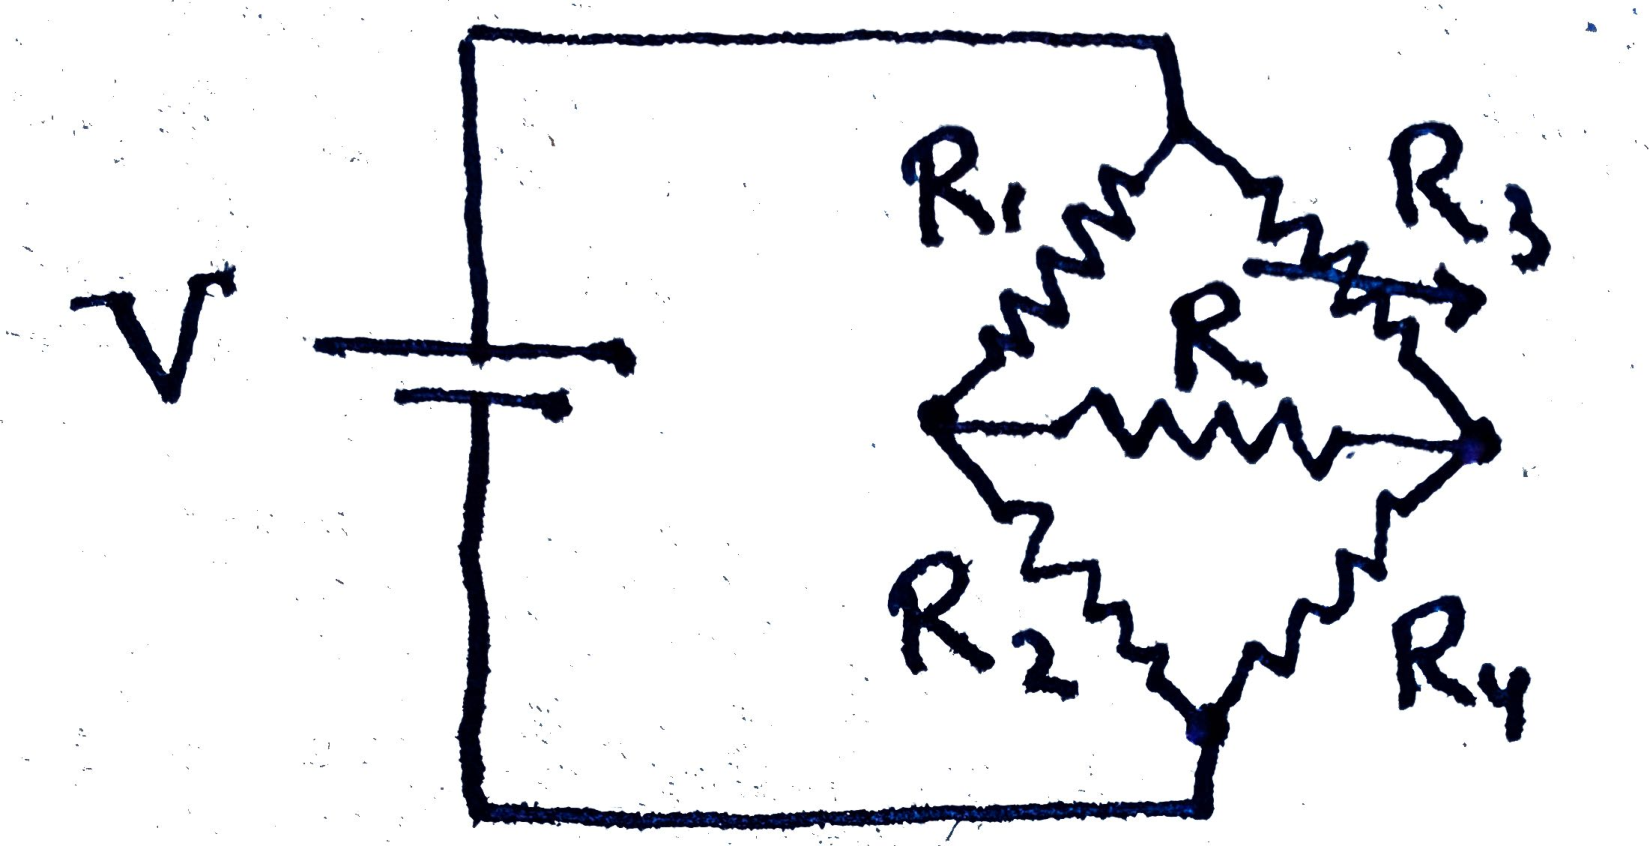
\includegraphics[width=\marginparwidth]{bridge.pdf}}

\paragraph{Problem~\theproblem:}\refstepcounter{problem}%
Imagine you have a tiny point charge $+q$ a small distance $h$ away
from a very large (much larger than $a$) planar conducting surface. Charge
will be induced on the conducting surface to make the electric field
perpendicular to the surface everywhere. This kind of problem is usually
solved by the method of images. Look up the method of images and
then write a vector expression for the electric field everywhere (outside
the conductor). Your expression might be ugly. Discuss with friends and
TAs for the simplest form.

\textsl{Bonus part, not for credit:} What is the induced charge
$\sigma$ on the conducting surface as a function of distance $r$ from
the closest point to the charge? How much total charge $Q$ is induced, if
you integrate over the whole surface?

\textsl{Bonus part, not for credit:} Why does the method of images work,
mathematically? You might want to think about mathematical concepts of
existence and uniqueness.

\paragraph{Problem~\theproblem:}\refstepcounter{problem}%
A laboratory function generator makes a voltage
\begin{equation}
V(t) = V_0\,\cos(\omega\,t)
\end{equation}
where $V_0$ is an amplitude, and $\omega$ is an angular frequency. Now
attach this function generator \emph{in parallel} to a resistor $R$ and
a capacitor $C$. What are the three currents running in the three different
legs of the circuit? That is, what is the current $I_V(t)$ coming out of the function
generator, the current $I_C(t)$ going into the capacitor, and the current $I_R(t)$ going
through the resistor? Each of these currents will be a function of time.

\textsl{Bonus part, not for credit:} What happens if you put the circuit
elements in series in a single loop? That's hard!

\end{document}
